\section{IMU (Inertial Measurement Unit)}
\label{sec:sec2_imu}

The IMU is a sensor that reports the linear acceleration and the angular velocity of a body by means of accelerometers and gyroscopes (sometimes also the orientation by means of magnetometers, but the IMU used did not have this capacity and therefore it is not analysed).

Starting with the gyroscope, and considering a single axis, it provides a measurement $\tilde{\omega}$ that relates to the angular velocity of that axis, and is given by Eq.\,\eqref{eq:sec2_meas_model_gyr}, which corresponds to the true angular velocity $\omega$ corrupted by the sensor bias $\omega_b$ and the sensor noise $\eta_{\omega}$, which is modelled as additive, zero-mean Gaussian noise.

\begin{equation}
    \label{eq:sec2_meas_model_gyr}
    \begin{split}
        \tilde{\omega} = \omega + \omega_b + \eta_\omega\\
        \eta_{\omega} \propto \sim N\left( 0, \sigma_{gyro}^2 \right)
    \end{split}
\end{equation}

In order to have 3FOF we use 3 gyroscopes, one for each orthogonal axis, and we assume no crosstalk between them. The bias is temperature dependent and can vary over time, but is generally modelled as a constant, and may be specified in the manufacturer's datasheet, alongside the sensor variance $\sigma_{gyro}^2$.

In order to obtain orientation information from angular velocity, we can integrate the angular velocity, as per the motion equations and corresponding Taylor expansion \eqref{eq:sec2_taylor_gyro}.

\begin{equation}
    \label{eq:sec2_taylor_gyro}
    \begin{split}
        \omega(t) = \frac{\partial}{\partial t} \theta(t) \\
        \theta(t+\delta t) \approx \theta(t) + \frac{\partial}{\partial t} \theta(t) \delta t + \epsilon\\
        \epsilon \propto O(\delta t^2)
    \end{split}
\end{equation}

A perfect measurement would produce a perfect estimation of orientation (apart from a constant offset). However, noise makes this more complicated, as shown in Fig.\,\ref{fig:sec2_gyr_noise_int}. Gaussian noise makes the orientation estimation fluctuate along the correct value, which may be acceptable in some situations. However, the bias poses a more complicated problem, as we are constantly integrating a wrong value, even when there is no movement.

\begin{figure}[H]
	\centering
		\begin{tabular}{cc}
		   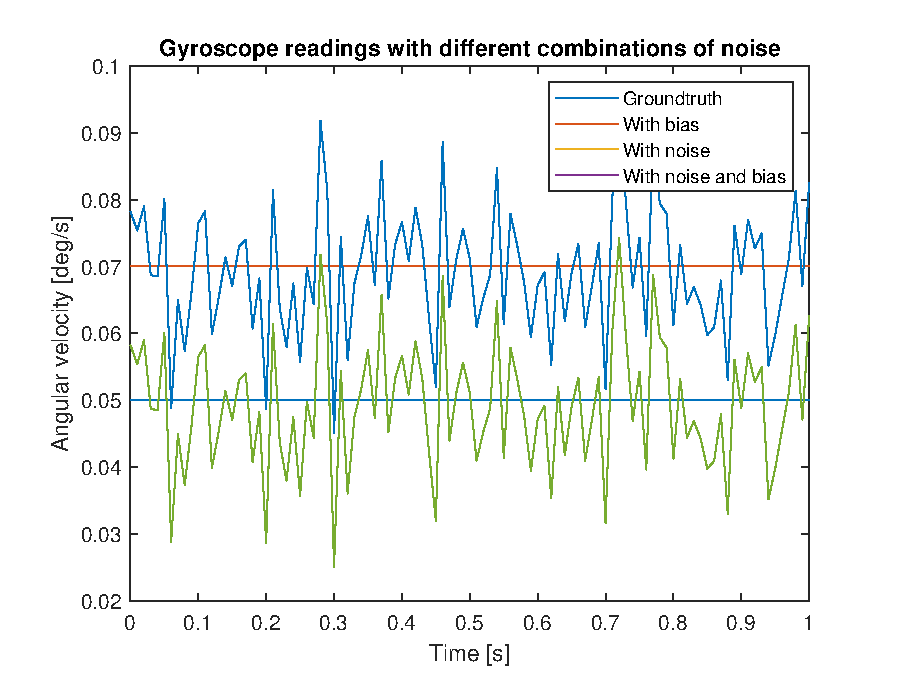
\includegraphics[width=0.45\linewidth]{gyr.eps} &
		   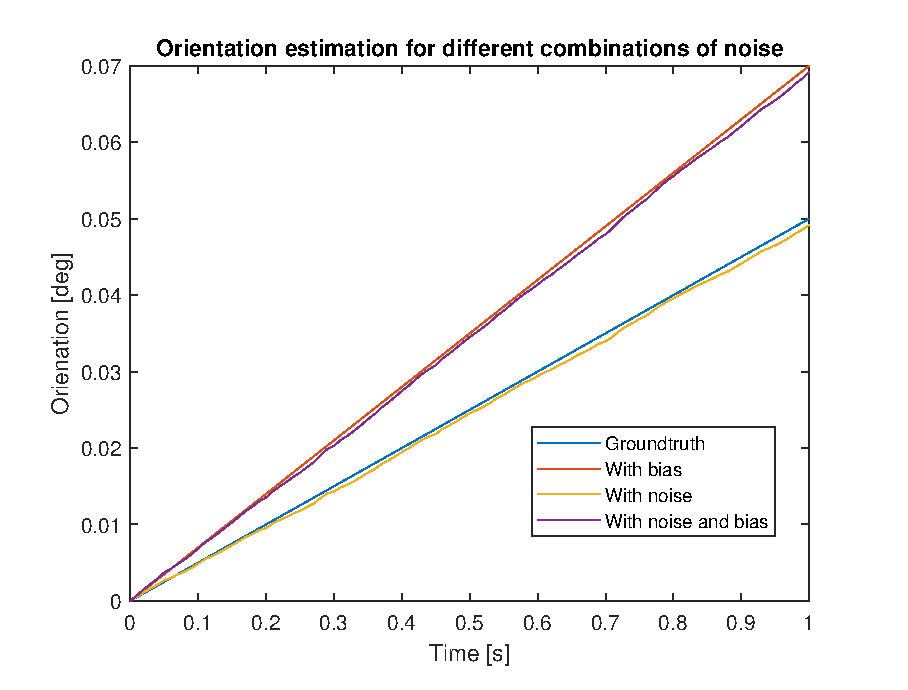
\includegraphics[width=0.45\linewidth]{or.eps} \\
		   (a) & (b) \\
		\end{tabular}
	\caption[Effect of noise on IMU]{(a) Effect of the various types of noise on the reading of the sensor and its impact on the estimation of the orientation (b)}   
    \label{fig:sec2_gyr_noise_int}
\end{figure}

Continuing with the accelerometers, a similar reasoning can be applied. We have a measurement $\tilde{a}$ given by Eq.\,\eqref{eq:sec2_meas_model_acc}, dependent on the true value $a$, sensor bias $a_b$ and noise $\eta_a$.

\begin{equation}
    \label{eq:sec2_meas_model_acc}
    \begin{split}
        \tilde{a} = a + a_b + \eta_a \\
        \eta_a \propto \sim N\left( 0, \sigma_{acc}^2 \right)
    \end{split}
\end{equation}

Again, a sensor for each axis is used, and no crosstalk is assumed. In order to obtain position information from angular velocity, we can integrate the acceleration twice (once for velocity and twice for position), as per the motion equations and corresponding Taylor expansion \eqref{eq:sec2_taylor_acc}.

\begin{equation}
    \label{eq:sec2_taylor_acc}
    \begin{split}
        v(t) = \frac{\partial}{\partial t} x(t) \\
        a(t) = \frac{\partial}{\partial t} v(t) = \frac{\partial^2}{\partial t^2} x(t)\\
        x(t+\delta t) \approx x(t) + \frac{\partial}{\partial t} x(t) \delta t + \frac{1 \partial^2}{2 \partial t^2} x(t) \delta t^2+ \epsilon\\
        \epsilon \propto O(\delta t^3)
    \end{split}
\end{equation}

Similarly, a perfect measurement would produce a perfect estimation of position (apart from a constant offset), but noise and bias render this task difficult. An extra step needs to be taken into account, which is the force of gravity, that needs to be subtracted from the affected axis (or axes, when no single axis is pointing straight down (or up)).

IMUs are very useful in the sense that they provide high speed information regarding both position and orientation (through angular veloxity and linear acceleration). However, the noisy measurements, coupled with the random walk associated with the bias, can lead to very incorrect estimations, especially when the system is standing still, and the noise overpowers the correct measurement itself.

\subsection{IMU calibration}

Just like the camera needs calibration, so do other sensors, in particular the IMU. In order to minimize the effect of noise and bias in the estimation, it is important to characterise these parameters. Ideally, they are supplied by the manufacturer in the datasheet. Oftentimes, however, they are not, and it is necessary to experimentally determine them.

We used the Kalibr framework \footnote{https://github.com/ethz-asl/kalibr} to characterise these parameters. \cite{board1998ieee} introduces the technique used by Kalibr, which consists of recording sensor measurement while standing still for a large amount of time (at least 4 hours), and then creating a plot with the log-log Allan deviation, as shown in Fig.\,\ref{fig:sec2_allan}. Two curves are then fitted to the plot, one with slope $-1/2$, and a second with slope $1/2$.

$\sigma_{gyro}$ and $\sigma_{acc}$ are taken directly at $\tau = 1$s, as we assume the noise power in most inertial sensors is dominated by noise at this frequency (point 1 in the plot). $\omega_b$ and $a_b$ corresponds to the value at which the line with slope $1/2$ crosses $\tau = 3$s (point 2 in the plot).

\begin{figure}[ht]
    \centering
    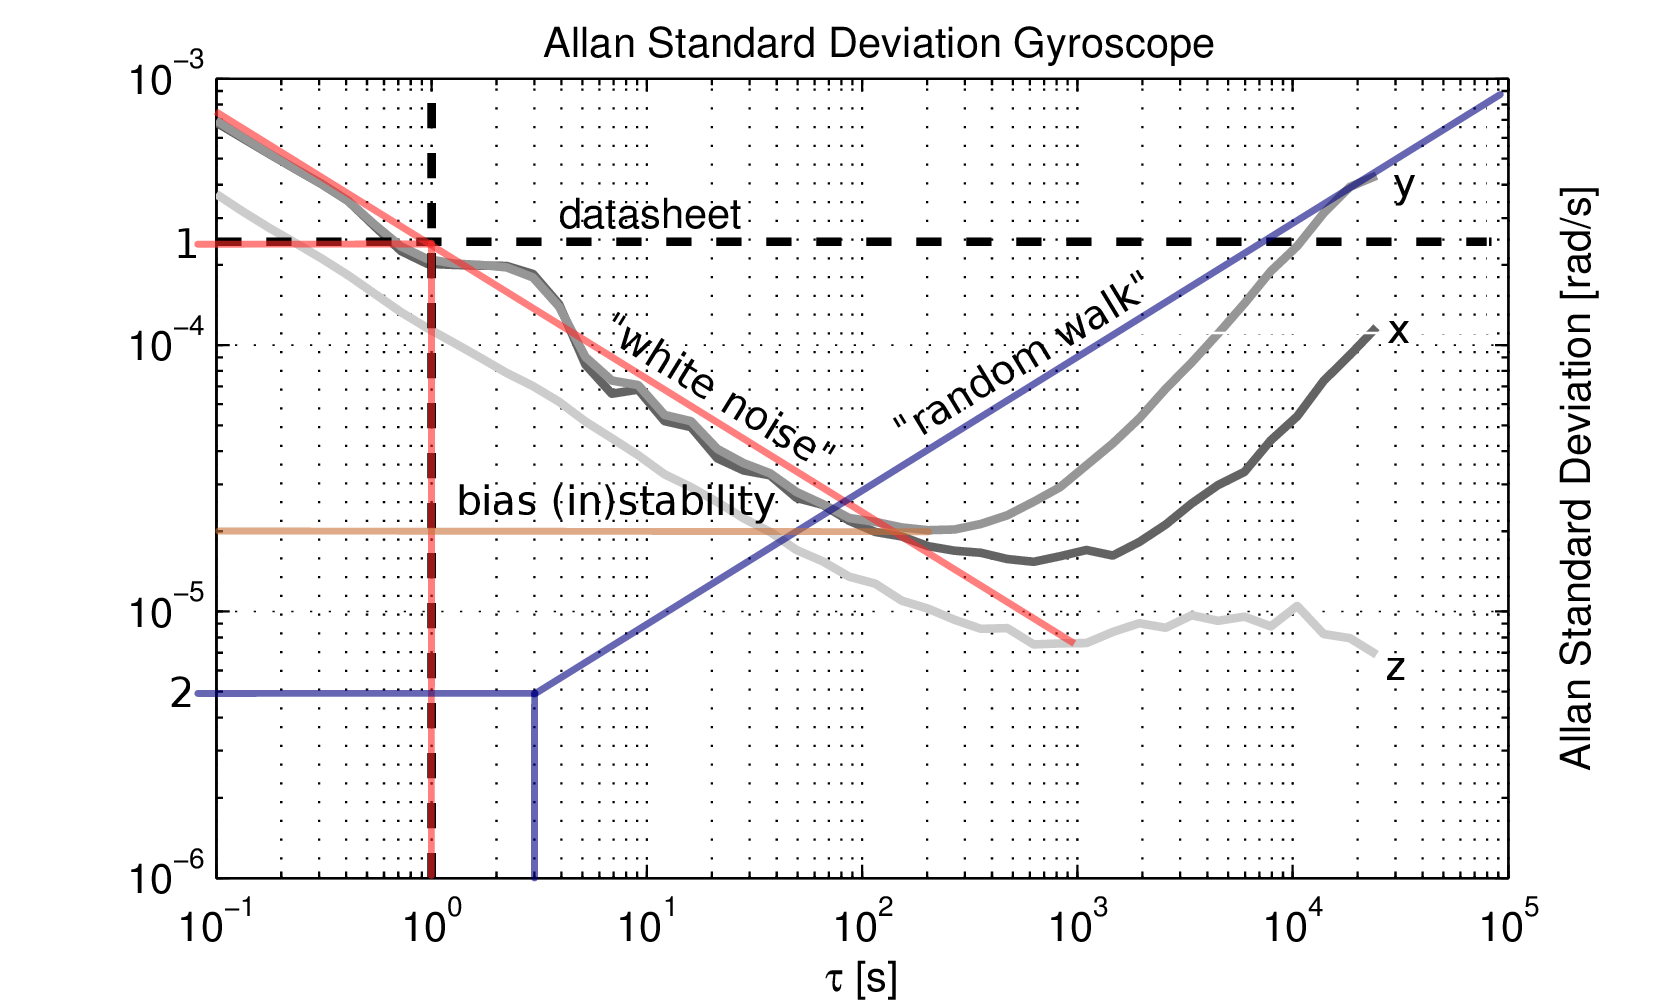
\includegraphics[width = 1\linewidth]{allan.png}
    \caption[Calibration of IMU through Allan standard deviation fitting]{Allan standard deviation of a gyroscope, showing the fitted lines, and noise characterisation, from the Kalibr wiki}
    \label{fig:sec2_allan}
\end{figure}
